\documentclass[12pt]{article}
\usepackage[utf8]{inputenc}
\usepackage{mathtools} % also loads amsmath
\usepackage{amsmath,amsthm,amsfonts,amssymb}
\usepackage{tikz}
% \usepackage{subfig}
\usepackage[english]{babel}
\usepackage{capt-of}
\usepackage{tabularray}
\usepackage{caption}
\usepackage{subcaption}
% \usepackage{subcaption}
% \captionsetup{compatibility=false}
\usepackage{graphicx}
\newtheorem{theorem}{Theorem}
\usetikzlibrary{calc}
\usetikzlibrary{shapes}
\usepackage{hyperref}
%might be unnecessary
\usepackage{doi}

%bibliography CMDS

%\usepackage{cite}
%\usepackage[style=alphabetic]{biblatex}
%\bibliographystyle{plain}

%\usepackage[style=alphabetic]{biblatex}

% \usepackage[backend=biber,style=alphabetic]{biblatex}
\usepackage[backend=biber,style=numeric]{biblatex}
% \usepackage[backend=biber,style=abbrv]{biblatex}
% \usepackage[backend=biber,style=alpha]{biblatex}
%\usepackage[backend=bibtex,style=alphabetic]{biblatex}
\addbibresource{./bibb.bib}

%%% With amsthm package, creates environments for nicely formatted,
%%% labeled, and numbered propositions, etc.
\theoremstyle{plain}

\newtheorem{thm}{Theorem}[section]
\newtheorem{lemma}[thm]{Lemma}
\newtheorem{prop}[thm]{Proposition}
\newtheorem{conj}[thm]{Conjecture}
\newtheorem{cor}[thm]{Corollary}
\newtheorem{claim}[thm]{Claim}
\newtheorem{fact}[thm]{Fact}
\newtheorem{constraint}[thm]{Constraint}
\newtheorem{condition}[thm]{Condition}

\theoremstyle{definition}
\newtheorem{eg}[thm]{Example}
% \newtheorem{defn}[thm]{Definition}
\newtheorem{definition}{Definition}[section]
\newtheorem{rem}[thm]{Remark}
\newtheorem{observ}[thm]{Observation}
\newtheorem{open}[thm]{Open Problem}
\newtheorem{prob.}[thm]{Problem}
\newtheorem{quest}[thm]{Question}

% I used these for making definitions and theorems, not what is above
\theoremstyle{remark}
\newtheorem{remark}[thm]{Remark}
\newtheorem{note}[thm]{Note}

\theoremstyle{definition}
% \newtheorem{definition}{Definition}[section]
\newtheorem{exmp}{Example}[section]

%custom commands

% blank cell
\newcommand{\cell}[4]{ \draw[thick] ( #1 , #2 ) rectangle ( #3 , #4 );}

% invisible cell for spacing
\newcommand{\spacecell}[4]{ \draw[thick, color=white] ( #1 , #2 ) rectangle ( #3 , #4 );}

% open cell 
\newcommand{\cellopen}[4]{ \draw[thick] ( #1 , #2 ) rectangle ( #3 , #4 ); \node[shape=circle,draw=red,fill=red, inner sep=0pt,minimum size=3pt] (A) at ( #1 * 0.5 + #3 * 0.5 , #2 * 0.5 + #4 * 0.5 ){};}
% /
% \newcommand{\cellA}[4]{ \draw[thick] ( #1 , #2 ) rectangle ( #3 , #4 ); \draw[red, thick, densely dotted] (#3 * 0.5 + #1 * 0.5 , #2) -- (#3, #4 * 0.5 + #2 * 0.5);}
% \
% \newcommand{\cellB}[4]{ \draw[thick] ( #1 , #2 ) rectangle ( #3 , #4 ); \draw[red, thick, densely dotted] (#3 * 0.5 + #1 * 0.5 , #2) -- (#1, #4 * 0.5 + #2 * 0.5);}
% /
% \newcommand{\cellC}[4]{ \draw[thick] ( #1 , #2 ) rectangle ( #3 , #4 ); \draw[red, thick, densely dotted] (#3 * 0.5 + #1 * 0.5 , #4) -- (#1, #4 * 0.5 + #2 * 0.5);}
% L
% \newcommand{\cellD}[4]{ \draw[thick] ( #1 , #2 ) rectangle ( #3 , #4 ); \draw[red, thick, densely dotted] (#3 * 0.5 + #1 * 0.5 , #4) -- (#3, #4 * 0.5 + #2 * 0.5);}
% |
% \newcommand{\cellE}[4]{ \draw[thick] ( #1 , #2 ) rectangle ( #3 , #4 ); \draw[red, thick, densely dotted] (#3 * 0.5 + #1 * 0.5 , #2) -- (#3 * 0.5 + #1 * 0.5 , #4);}
% % -
% \newcommand{\cellF}[4]{ \draw[thick] ( #1 , #2 ) rectangle ( #3 , #4 ); \draw[red, thick, densely dotted] (#3, #4 * 0.5 + #2 * 0.5) -- (#1, #4 * 0.5 + #2 * 0.5);}

% \newcommand{\cellAf}[4]{\filldraw[gray!40] ( #1 , #2 ) rectangle ( #3 , #4 ); \draw[thick] ( #1 , #2 ) rectangle ( #3 , #4 ); \draw[red, thick, densely dotted] (#3 * 0.5 + #1 * 0.5 , #2) -- (#3, #4 * 0.5 + #2 * 0.5);}
% \
% \newcommand{\cellBf}[4]{\filldraw[gray!40] ( #1 , #2 ) rectangle ( #3 , #4 ); \draw[thick] ( #1 , #2 ) rectangle ( #3 , #4 ); \draw[red, thick, densely dotted] (#3 * 0.5 + #1 * 0.5 , #2) -- (#1, #4 * 0.5 + #2 * 0.5);}
% /
% \newcommand{\cellCf}[4]{\filldraw[gray!40] ( #1 , #2 ) rectangle ( #3 , #4 ); \draw[thick] ( #1 , #2 ) rectangle ( #3 , #4 ); \draw[red, thick, densely dotted] (#3 * 0.5 + #1 * 0.5 , #4) -- (#1, #4 * 0.5 + #2 * 0.5);}
% L
% \newcommand{\cellDf}[4]{\filldraw[gray!40] ( #1 , #2 ) rectangle ( #3 , #4 ); \draw[thick] ( #1 , #2 ) rectangle ( #3 , #4 ); \draw[red, thick, densely dotted] (#3 * 0.5 + #1 * 0.5 , #4) -- (#3, #4 * 0.5 + #2 * 0.5);}
% |
% \newcommand{\cellEf}[4]{\filldraw[gray!40] ( #1 , #2 ) rectangle ( #3 , #4 ); \draw[thick] ( #1 , #2 ) rectangle ( #3 , #4 ); \draw[red, thick, densely dotted] (#3 * 0.5 + #1 * 0.5 , #2) -- (#3 * 0.5 + #1 * 0.5 , #4);}
% % -
% \newcommand{\cellFf}[4]{\filldraw[gray!40] ( #1 , #2 ) rectangle ( #3 , #4 ); \draw[thick] ( #1 , #2 ) rectangle ( #3 , #4 ); \draw[red, thick, densely dotted] (#3, #4 * 0.5 + #2 * 0.5) -- (#1, #4 * 0.5 + #2 * 0.5);}


\newcommand{\cellA}[4]{\draw[red, thick, densely dotted] ( #1 + 0.5 , #2 ) arc(0:90:{0.5}); \draw[thick] ( #1 , #2 ) rectangle ( #3 , #4 );}
\newcommand{\cellB}[4]{\draw[red, thick, densely dotted] ( #1 + 1 , #2 + 0.5 ) arc(90:180:{0.5}); \draw[thick] ( #1 , #2 ) rectangle ( #3 , #4 );}
\newcommand{\cellC}[4]{\draw[red, thick, densely dotted] ( #1 + 0.5, #2 + 1 ) arc(180:270:{0.5}); \draw[thick] ( #1 , #2 ) rectangle ( #3 , #4 );}
\newcommand{\cellD}[4]{\draw[red, thick, densely dotted] ( #1 , #2 + 0.5 ) arc(-90:0:{0.5}); \draw[thick] ( #1 , #2 ) rectangle ( #3 , #4 );}
\newcommand{\cellE}[4]{\draw[red, thick, densely dotted] (#3, #4 * 0.5 + #2 * 0.5) -- (#1, #4 * 0.5 + #2 * 0.5); \draw[thick] ( #1 , #2 ) rectangle ( #3 , #4 );}
\newcommand{\cellF}[4]{\draw[red, thick, densely dotted] (#3 * 0.5 + #1 * 0.5 , #2) -- (#3 * 0.5 + #1 * 0.5 , #4); \draw[thick] ( #1 , #2 ) rectangle ( #3 , #4 );}
\newcommand{\cellG}[4]{\draw[red, thick, densely dotted] ( #1 + 0.5 , #2 ) arc(0:90:{0.5}); \draw[red, thick, densely dotted] ( #1 + 0.5, #2 + 1 ) arc(180:270:{0.5}); \draw[thick] ( #1 , #2 ) rectangle ( #3 , #4 );}
\newcommand{\cellH}[4]{\draw[red, thick, densely dotted] ( #1 , #2 + 0.5 ) arc(-90:0:{0.5}); \draw[red, thick, densely dotted] ( #1 + 1 , #2 + 0.5 ) arc(90:180:{0.5}); \draw[thick] ( #1 , #2 ) rectangle ( #3 , #4 );}
\newcommand{\cellI}[4]{\draw[red, thick, densely dotted] (#3 * 0.5 + #1 * 0.5 , #2) -- (#3 * 0.5 + #1 * 0.5 , #4); \node[shape=circle,draw=none,fill=white, inner sep=3pt,minimum size=5pt] (A) at ( #1 + 0.5 , #2 + 0.5 ) {}; \draw[red, thick, densely dotted] (#3, #4 * 0.5 + #2 * 0.5) -- (#1, #4 * 0.5 + #2 * 0.5); \draw[thick] ( #1 , #2 ) rectangle ( #3 , #4 );}
\newcommand{\cellJ}[4]{\draw[red, thick, densely dotted] (#3, #4 * 0.5 + #2 * 0.5) -- (#1, #4 * 0.5 + #2 * 0.5); \node[shape=circle,draw=none,fill=white, inner sep=3pt,minimum size=5pt] (A) at ( #1 + 0.5 , #2 + 0.5 ) {}; \draw[thick] ( #1 , #2 ) rectangle ( #3 , #4 ); \draw[red, thick, densely dotted] (#3 * 0.5 + #1 * 0.5 , #2) -- (#3 * 0.5 + #1 * 0.5 , #4);}


\newcommand{\cellAf}[4]{\filldraw[gray!40] ( #1 , #2 ) rectangle ( #3 , #4 ); \draw[red, thick, densely dotted] ( #1 + 0.5 , #2 ) arc(0:90:{0.5}); \draw[thick] ( #1 , #2 ) rectangle ( #3 , #4 );}
\newcommand{\cellBf}[4]{\filldraw[gray!40] ( #1 , #2 ) rectangle ( #3 , #4 ); \draw[red, thick, densely dotted] ( #1 + 1 , #2 + 0.5 ) arc(90:180:{0.5}); \draw[thick] ( #1 , #2 ) rectangle ( #3 , #4 );}
\newcommand{\cellCf}[4]{\filldraw[gray!40] ( #1 , #2 ) rectangle ( #3 , #4 ); \draw[red, thick, densely dotted] ( #1 + 0.5, #2 + 1 ) arc(180:270:{0.5}); \draw[thick] ( #1 , #2 ) rectangle ( #3 , #4 );}
\newcommand{\cellDf}[4]{\filldraw[gray!40] ( #1 , #2 ) rectangle ( #3 , #4 ); \draw[red, thick, densely dotted] ( #1 , #2 + 0.5 ) arc(-90:0:{0.5}); \draw[thick] ( #1 , #2 ) rectangle ( #3 , #4 );}
\newcommand{\cellEf}[4]{\filldraw[gray!40] ( #1 , #2 ) rectangle ( #3 , #4 ); \draw[red, thick, densely dotted] (#3, #4 * 0.5 + #2 * 0.5) -- (#1, #4 * 0.5 + #2 * 0.5); \draw[thick] ( #1 , #2 ) rectangle ( #3 , #4 );}
\newcommand{\cellFf}[4]{\filldraw[gray!40] ( #1 , #2 ) rectangle ( #3 , #4 ); \draw[red, thick, densely dotted] (#3 * 0.5 + #1 * 0.5 , #2) -- (#3 * 0.5 + #1 * 0.5 , #4); \draw[thick] ( #1 , #2 ) rectangle ( #3 , #4 );}
\newcommand{\cellGf}[4]{\filldraw[gray!40] ( #1 , #2 ) rectangle ( #3 , #4 ); \draw[red, thick, densely dotted] ( #1 + 0.5 , #2 ) arc(0:90:{0.5}); \draw[red, thick, densely dotted] ( #1 + 0.5, #2 + 1 ) arc(180:270:{0.5}); \draw[thick] ( #1 , #2 ) rectangle ( #3 , #4 );}
\newcommand{\cellHf}[4]{\filldraw[gray!40] ( #1 , #2 ) rectangle ( #3 , #4 ); \draw[red, thick, densely dotted] ( #1 , #2 + 0.5 ) arc(-90:0:{0.5}); \draw[red, thick, densely dotted] ( #1 + 1 , #2 + 0.5 ) arc(90:180:{0.5}); \draw[thick] ( #1 , #2 ) rectangle ( #3 , #4 );}
\newcommand{\cellIf}[4]{\filldraw[gray!40] ( #1 , #2 ) rectangle ( #3 , #4 ); \draw[red, thick, densely dotted] (#3 * 0.5 + #1 * 0.5 , #2) -- (#3 * 0.5 + #1 * 0.5 , #4); \node[shape=circle,draw=none,fill=gray!40, inner sep=3pt,minimum size=5pt] (A) at ( #1 + 0.5 , #2 + 0.5 ) {}; \draw[red, thick, densely dotted] (#3, #4 * 0.5 + #2 * 0.5) -- (#1, #4 * 0.5 + #2 * 0.5); \draw[thick] ( #1 , #2 ) rectangle ( #3 , #4 );}
\newcommand{\cellJf}[4]{\filldraw[gray!40] ( #1 , #2 ) rectangle ( #3 , #4 ); \draw[red, thick, densely dotted] (#3, #4 * 0.5 + #2 * 0.5) -- (#1, #4 * 0.5 + #2 * 0.5); \node[shape=circle,draw=none,fill=gray!40, inner sep=3pt,minimum size=5pt] (A) at ( #1 + 0.5 , #2 + 0.5 ) {}; \draw[thick] ( #1 , #2 ) rectangle ( #3 , #4 ); \draw[red, thick, densely dotted] (#3 * 0.5 + #1 * 0.5 , #2) -- (#3 * 0.5 + #1 * 0.5 , #4);}


\newcommand{\lablnode}[3]{\node[shape=circle,draw=none,fill=none, inner sep=0pt,minimum size=0pt] (A) at ( #1 , #2 ) {#3};}
\newcommand{\lablvertex}[3]{\node[shape=circle,draw=none,fill=white, inner sep=2pt,minimum size=5pt] (A) at ( #1 , #2 ) {#3};}

\usepackage[margin=1in]{geometry}
\date{}
%doc info
\author{
    \textbf{Jack Hanke}\\
    Northwestern University
    \and
    % \textbf{Michael Maltenfort}\\
    % Northwestern University
    % \and
    \textbf{Richard Schank}\\
    }
\title{\textbf{Enumeration of Messy Knot Mosaics}}
% \date{\today}

\begin{document}
\maketitle

\begin{center}

    \begin{abstract}
        Lomonaco and Kauffman introduced a system of mosaics to model quantum knots. These systems of mosaics are composed of an $m \times n$ rectangular grid of $11$ possible tiles. Oh and colleagues introduced a state matrix recursion method to exactly enumerate a subset of these mosaics that have the property of being suitably connected, which they call knot mosaics. We introduce and enumerate mosaics with the related property in which only some tiles must be suitably connected, which we call messy knot mosaics.
    \end{abstract}

\end{center}

\section{Introduction}

Lomonaco and Kauffman \cite{Lomonaco08} introduced a model for quantum knots in which an $m \times n$ matrix is constructed using $11$ distinct symbols called \textit{tiles}. These tiles, diagrammed below, are composed of unit squares with dotted lines connecting $2$ or $4$ sides at their midpoint.

\begin{center}
    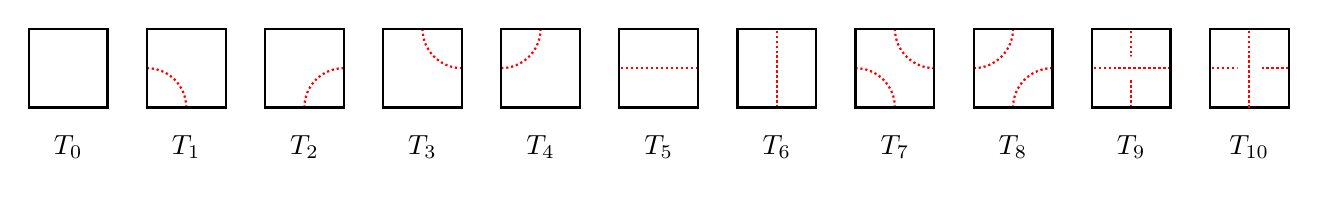
\begin{tikzpicture}
        \cell{0}{0}{1}{1}
        \( \lablnode{0.5}{-0.5}{$T_0$} \) 
        \cellA{1.5}{0}{2.5}{1}
        \( \lablnode{2}{-0.5}{$T_1$} \) 
        \cellB{3}{0}{4}{1}
        \( \lablnode{3.5}{-0.5}{$T_2$} \) 
        \cellC{4.5}{0}{5.5}{1}
        \( \lablnode{5}{-0.5}{$T_3$} \) 
        \cellD{6}{0}{7}{1}
        \( \lablnode{6.5}{-0.5}{$T_4$} \) 
        \cellE{7.5}{0}{8.5}{1}
        \( \lablnode{8}{-0.5}{$T_5$} \) 
        \cellF{9}{0}{10}{1}
        \( \lablnode{9.5}{-0.5}{$T_6$} \) 
        \cellG{10.5}{0}{11.5}{1}
        \( \lablnode{11}{-0.5}{$T_7$} \) 
        \cellH{12}{0}{13}{1}
        \( \lablnode{12.5}{-0.5}{$T_8$} \) 
        \cellI{13.5}{0}{14.5}{1}
        \( \lablnode{14}{-0.5}{$T_{9}$} \) 
        \cellJ{15}{0}{16}{1}
        \( \lablnode{15.5}{-0.5}{$T_{10}$} \) 
    \end{tikzpicture}
\end{center}

We denote the set of tiles $\mathbb{T}=\{T_0, \dots, T_{10}\}$. A \textit{mosaic} of size $(m,n)$ is an $m \times n$ matrix made up of elements from $\mathbb{T}$. Figure \ref{fig:example mosaic} shows an example mosaic of size $(5,7)$. We denote the set of all mosaics of size $(m,n)$ as $\mathbb{M}^{(m,n)}$. As there are $11$ elements in $\mathbb{T}$, there are $11^{mn}$ mosaics in $\mathbb{M}^{(m,n)}$. A \textit{mosaic system} is then a subset of $\mathbb{M}^{(m,n)}$ with some property. 

\begin{figure}[h!]
    \begin{center}
    \begin{subfigure}{0.4\textwidth}
        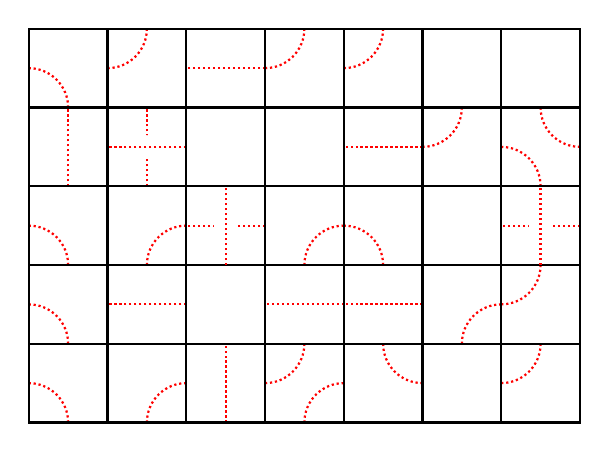
\begin{tikzpicture}
        % row1
        \cellA{0}{0}{1}{1}
        \cellB{1}{0}{2}{1}
        \cellF{2}{0}{3}{1}
        \cellH{3}{0}{4}{1}
        \cellC{4}{0}{5}{1}
        \cell{5}{0}{6}{1}
        \cellD{6}{0}{7}{1}
        % row2
        \cellA{0}{1}{1}{2}
        \cellE{1}{1}{2}{2}
        \cell{2}{1}{3}{2}
        \cellE{3}{1}{4}{2}
        \cellE{4}{1}{5}{2}
        \cellB{5}{1}{6}{2}
        \cellD{6}{1}{7}{2}
        % row3
        \cellA{0}{2}{1}{3}
        \cellB{1}{2}{2}{3}
        \cellJ{2}{2}{3}{3}
        \cellB{3}{2}{4}{3}
        \cellA{4}{2}{5}{3}
        \cell{5}{2}{6}{3}
        \cellJ{6}{2}{7}{3}
        % row4
        \cellF{0}{3}{1}{4}
        \cellI{1}{3}{2}{4}
        \cell{2}{3}{3}{4}
        \cell{3}{3}{4}{4}
        \cellE{4}{3}{5}{4}
        \cellD{5}{3}{6}{4}
        \cellG{6}{3}{7}{4}
        % row5
        \cellA{0}{4}{1}{5}
        \cellD{1}{4}{2}{5}
        \cellE{2}{4}{3}{5}
        \cellD{3}{4}{4}{5}
        \cellD{4}{4}{5}{5}
        \cell{5}{4}{6}{5}
        \cell{6}{4}{7}{5}
        \end{tikzpicture}
    \caption{A mosaic}
    \label{fig:example mosaic}
    \end{subfigure}
% \hfill
\hspace{0.05\textwidth}
\begin{subfigure}{0.4\textwidth}
    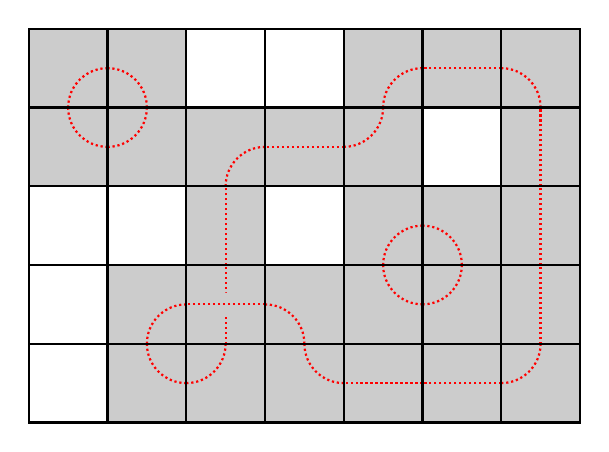
\begin{tikzpicture}
        % row1
        \cell{0}{0}{1}{1}
        \cellCf{1}{0}{2}{1}
        \cellDf{2}{0}{3}{1}
        \cellCf{3}{0}{4}{1}
        \cellEf{4}{0}{5}{1}
        \cellEf{5}{0}{6}{1}
        \cellDf{6}{0}{7}{1}
        % row2
        \cell{0}{1}{1}{2}
        \cellBf{1}{1}{2}{2}
        \cellIf{2}{1}{3}{2}
        \cellAf{3}{1}{4}{2}
        \cellCf{4}{1}{5}{2}
        \cellDf{5}{1}{6}{2}
        \cellFf{6}{1}{7}{2}
        % row3
        \cell{0}{2}{1}{3}
        \cell{1}{2}{2}{3}
        \cellFf{2}{2}{3}{3}
        \cell{3}{2}{4}{3}
        \cellBf{4}{2}{5}{3}
        \cellAf{5}{2}{6}{3}
        \cellFf{6}{2}{7}{3}
        % row4
        \cellCf{0}{3}{1}{4}
        \cellDf{1}{3}{2}{4}
        \cellBf{2}{3}{3}{4}
        \cellEf{3}{3}{4}{4}
        \cellDf{4}{3}{5}{4}
        \cell{5}{3}{6}{4}
        \cellFf{6}{3}{7}{4}
        % row5
        \cellBf{0}{4}{1}{5}
        \cellAf{1}{4}{2}{5}
        \cell{2}{4}{3}{5}
        \cell{3}{4}{4}{5}
        \cellBf{4}{4}{5}{5}
        \cellEf{5}{4}{6}{5}
        \cellAf{6}{4}{7}{5}
    \end{tikzpicture}
    \caption{A knot mosaic}
    \label{fig:example knot mosaic}
\end{subfigure}

\end{center}
\caption{Examples of mosaics of size $(5,7)$ made of tiles in $\mathbb{T}$}
\label{fig:example mosaics}
\end{figure}

We are interested in mosaics with the property of being \textit{suitably connected}, which is defined as follows. Consider an edge shared between two tiles in Figure \ref{fig:example mosaic}. The edge has either $0$, $1$, or $2$ dotted lines drawn from its midpoint. Also note that the edges of the tiles on the boundary of the matrix are not shared by another tile. Therefore these edges only have $0$ or $1$ dotted lines drawn from their midpoint. A mosaic is suitably connected if all edges have $0$ or $2$ dotted lines drawn from their midpoint.

Lomonaco and Kauffman \cite{Lomonaco08} call these \textit{knot mosaics} because, other than the mosaic consisting of all $T_0$ tiles, the dotted lines form  \textit{knots}. Following the notation in \cite{Oh2014} we denote the subset of mosaics of size $(m,n)$ that are knot mosaics as $\mathbb{K}^{(m,n)}$. Figure \ref{fig:example knot mosaic} shows a knot mosaic of size $(5,7)$ that contains $3$ knots, with the tiles that make up the knots highlighted in gray. Note that a mosaic can contain knots isomorphic to the unknot, as well as knots that encompass other knots. 

Let $k_{m,n} = |\mathbb{K}^{(m,n)}|$ be the number of knot mosaics of size $(m,n)$. First notice that if either $m$ or $n$ is $1$, one can only construct a knot mosaic using $T_0$ tiles, so $k_{m,1} = k_{1,n} = 1.$ Oh et al. \cite{Oh2014} showed the following for $m,n \geq 2$.

\begin{thm}[\cite{Oh2014}]
    \label{thm:Oh2014}
    The number of knot mosaics of size $(m,n)$ for $m,n \geq 2$ is $k_{m,n} = 2 \left\| (X_{m-2}+O_{m-2})^{n-2} \right\|$, where $X_{m-2}$ and $O_{m-2}$ are $2^{m-2} \times 2^{m-2}$ matrices defined as

    $$ X_{k+1} = \begin{bmatrix}
        X_k & O_k \\
        O_k & X_k
    \end{bmatrix}
    \text{ and }
    O_{k+1} = \begin{bmatrix}
        O_k & X_k \\
        X_k & 4O_k
    \end{bmatrix}, $$
    
    for $k=0,1,\dots,m-3$, and $X_0 = O_0 = \begin{bmatrix} 1 \\ \end{bmatrix}$. Here $\left\| N \right\|$ denotes the sum of elements of matrix $N$.
\end{thm}

Oh and colleagues refer to these matrices $X_k$ and $O_k$ as \textit{state matrices}. The authors utilize this state matrix recursion to bound the growth rate of knot mosaics $\delta = \lim_{n \to \infty} k_{n,n}^{\frac{1}{n^2}}$ \cite{Oh2016, Oh2019, Choi2024}, and Oh further adapts the method to solve problems in monomer and dimer tilings \cite{Oh2018Aztec, Oh2019tiling}. An unexamined direction in this research program is modifying the suitably connected property. This motivates us to introduce \textit{messy knot mosaics}.


\section{Messy Knot Mosaics}\label{section:messy mosaics}

\begin{definition}
    A \textit{messy knot mosaic} is a mosaic that contains at least one knot. 
\end{definition}

Figure \ref{fig:messy mosaic example} shows two examples of messy knot mosaic of size $(5,7)$ that contains $3$ knots\footnote{Certain permutations of $\{T_1, T_2, T_3, T_4\}$ and $\{T_7,T_8\}$ can make shapes that appear to be knots but have hanging connections, as seen in the $(0,4)$ position in the right example in Figure \ref{fig:messy mosaic example}. These are not considered knots by this paper and all referenced works.}, with the tiles that make up the knots highlighted in gray. All knot mosaics are messy knot mosaics.

\begin{figure}[h!]
    \begin{center}

\begin{subfigure}{0.4\textwidth}
    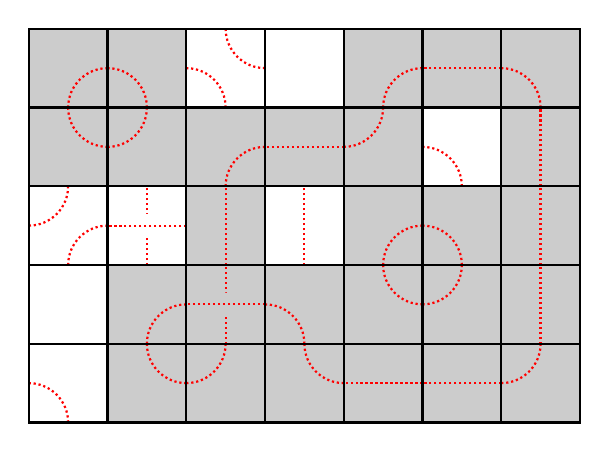
\begin{tikzpicture}
       % row1
        \cellA{0}{0}{1}{1}
        \cellCf{1}{0}{2}{1}
        \cellDf{2}{0}{3}{1}
        \cellCf{3}{0}{4}{1}
        \cellEf{4}{0}{5}{1}
        \cellEf{5}{0}{6}{1}
        \cellDf{6}{0}{7}{1}
        % row2
        \cell{0}{1}{1}{2}
        \cellBf{1}{1}{2}{2}
        \cellIf{2}{1}{3}{2}
        \cellAf{3}{1}{4}{2}
        \cellCf{4}{1}{5}{2}
        \cellDf{5}{1}{6}{2}
        \cellFf{6}{1}{7}{2}
        % row3
        \cellH{0}{2}{1}{3}
        \cellI{1}{2}{2}{3}
        \cellFf{2}{2}{3}{3}
        \cellF{3}{2}{4}{3}
        \cellBf{4}{2}{5}{3}
        \cellAf{5}{2}{6}{3}
        \cellFf{6}{2}{7}{3}
        % row4
        \cellCf{0}{3}{1}{4}
        \cellDf{1}{3}{2}{4}
        \cellBf{2}{3}{3}{4}
        \cellEf{3}{3}{4}{4}
        \cellDf{4}{3}{5}{4}
        \cellA{5}{3}{6}{4}
        \cellFf{6}{3}{7}{4}
        % row5
        \cellBf{0}{4}{1}{5}
        \cellAf{1}{4}{2}{5}
        \cellG{2}{4}{3}{5}
        \cell{3}{4}{4}{5}
        \cellBf{4}{4}{5}{5}
        \cellEf{5}{4}{6}{5}
        \cellAf{6}{4}{7}{5}
    \end{tikzpicture}
\end{subfigure}
% \hfill
\hspace{0.05\textwidth}
\begin{subfigure}{0.4\textwidth}
        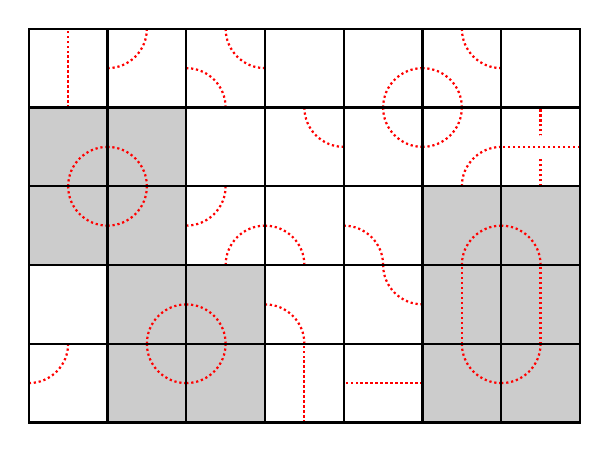
\begin{tikzpicture}
        % row1
        \cellD{0}{0}{1}{1}
        \cellCf{1}{0}{2}{1}
        \cellDf{2}{0}{3}{1}
        \cellF{3}{0}{4}{1}
        \cellE{4}{0}{5}{1}
        \cellCf{5}{0}{6}{1}
        \cellDf{6}{0}{7}{1}
        % row2
        \cell{0}{1}{1}{2}
        \cellBf{1}{1}{2}{2}
        \cellAf{2}{1}{3}{2}
        \cellA{3}{1}{4}{2}
        \cellC{4}{1}{5}{2}
        \cellFf{5}{1}{6}{2}
        \cellFf{6}{1}{7}{2}
        % row3
        \cellCf{0}{2}{1}{3}
        \cellDf{1}{2}{2}{3}
        \cellH{2}{2}{3}{3}
        \cellA{3}{2}{4}{3}
        \cellA{4}{2}{5}{3}
        \cellBf{5}{2}{6}{3}
        \cellAf{6}{2}{7}{3}
        % row4
        \cellBf{0}{3}{1}{4}
        \cellAf{1}{3}{2}{4}
        \cell{2}{3}{3}{4}
        \cellC{3}{3}{4}{4}
        \cellC{4}{3}{5}{4}
        \cellH{5}{3}{6}{4}
        \cellI{6}{3}{7}{4}
        % row5
        \cellF{0}{4}{1}{5}
        \cellD{1}{4}{2}{5}
        \cellG{2}{4}{3}{5}
        \cell{3}{4}{4}{5}
        \cellB{4}{4}{5}{5}
        \cellG{5}{4}{6}{5}
        \cell{6}{4}{7}{5}
    \end{tikzpicture}
\end{subfigure}

\end{center}
\caption{Messy knot mosaics}
\label{fig:messy mosaic example}
\end{figure}

It turns out to be simpler to enumerate the number of mosaics that \textit{do not} contain a knot. Therefore, let $\mathbb{S}^{(m,n)}$ be the set of mosaics that do not contain a knot, and let $|\mathbb{S}^{(m,n)}| = s_{m,n}$. Clearly the number of messy knot mosaics is then $11^{mn} - s_{m,n}$.

From the fact that the smallest knot is made of four tiles, shown in Figure \ref{fig:smallest knot}, we can then conclude that $s_{n,1}=11^n$, and $s_{2,2} = 11^4 - 1$. For $n,m \geq 2$, we first define the state matrices for messy knot mosaics.

\begin{figure}[h!]
    \begin{center}
    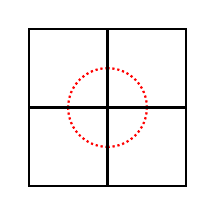
\begin{tikzpicture}
        % row1
        \cellC{0}{0}{1}{1}
        \cellD{1}{0}{2}{1}
        % row2
        \cellB{0}{1}{1}{2}
        \cellA{1}{1}{2}{2}
    \end{tikzpicture}
    \end{center}
    \caption{The smallest knot}
    \label{fig:smallest knot}
\end{figure}

\begin{definition}

Define $A(2) = \begin{bmatrix}
11^2 & 1 \\
-1 & 1
\end{bmatrix}$. We recursively define $A(k+1) \in \mathbb{N}^{2^{k} \times 2^{k}}$ given $A(k)$. Begin by writing
$
A(k) = \begin{bmatrix}
A_{0,0} & A_{0,1} \\
A_{1,0} & A_{1,1}
\end{bmatrix}
$, where the block matrices $A_{i,j}$ are square block matrices of size $2^{k-1} \times 2^{k-1}$. We then have

$$
A(k+1) = \begin{bmatrix}
    11A_{0,0} & \frac{1}{11}A_{0,0} & 11A_{0,1} & A_{0,1} \\
    -\frac{1}{11}A_{0,0} & \frac{1}{11}A_{0,0} & 4A_{0,1} & A_{0,1} \\
    11A_{1,0} & -4A_{1,0} & 11A_{1,1}  & A_{1,1} \\
    A_{1,0} & -A_{1,0} & A_{1,1} & 11A_{1,1} \\
\end{bmatrix}.
$$

Construct $A(m)$ by starting with $k=2$ and recursing until $k=m$. 

\end{definition}

\begin{thm}
\label{thm: messy mosaics}
The number of mosaics of size $(m,n)$ that \textit{do not} contain a knot is the $(0,0)$ entry of $A(m)^n$.
\end{thm}

\section{Preliminaries}

We begin by defining a mapping $f$ between $\mathbb{M}^{(m,n)}$ to a \textit{binary lattice} of size $(m,n)$. A binary lattice of size $(m,n)$ is a rectangular lattice of $m+1$ by $n+1$ vertices, in which the boundary vertices are labeled $0$, and the interior vertices are either $0$ or $1$. An example of a binary lattice of size $(5,7)$ is shown on the right of Figure \ref{fig:example of f mapping}. Also let $\mathbb{L}^{(m,n)}$ be the set of all binary lattices of size $(m,n)$, which gives $\left|\mathbb{L}^{(m,n)}\right| = 2^{(m-1)(n-1)}$. 

\begin{definition}

$f: \mathbb{M}^{(m,n)} \to \mathbb{L}^{(m,n)}$ takes a mosaic and labels each vertex with the following rule. If the vertex is surrounded by an even number of knots (including $0$ knots), label it $0$. If the vertex is surrounded by an odd number of knots, label it $1$. Removing the red dotted lines from the tiles gives the binary lattice. 
    
\end{definition}

Similarly, define the \textit{preimage} of a set $L$ under $f$ to be

$$f^{-1}(L) = \{m \in \mathbb{M}^{(m,n)} | f(m) \in L\}.$$

We want to compute $s_{m,n}$ by computing $f^{-1}(\{\ell\})$ for each $\ell \in \mathbb{L}^{(m,n)}$, and then summing over all $\ell$. We begin by finding a simple way to compute $f^{-1}(\ell)$ for a binary lattice $\ell$ by examining the structure of $\ell$.

\begin{figure}
\begin{center}
    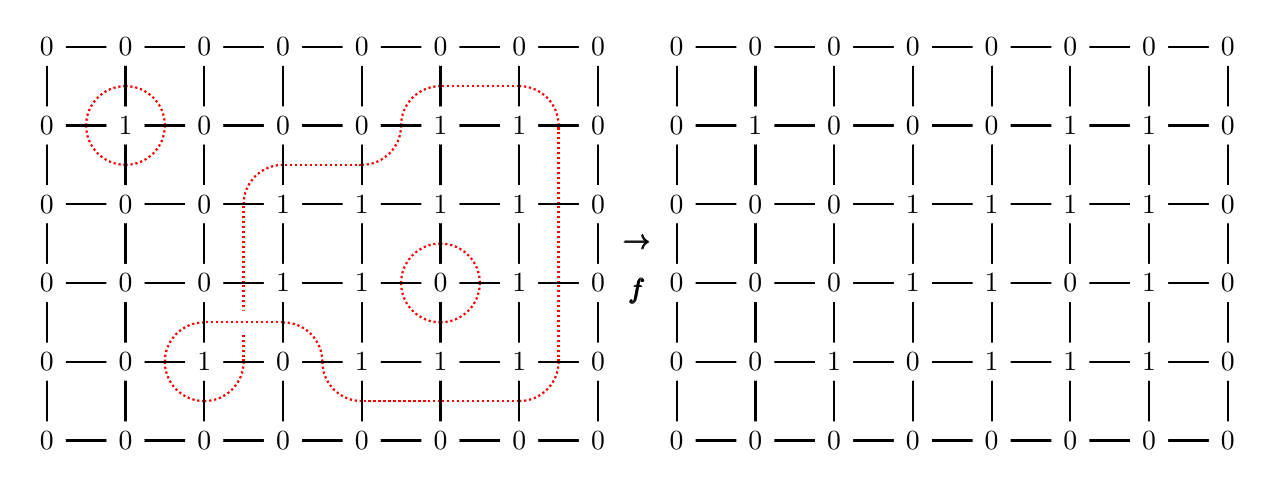
\begin{tikzpicture}
        % row1
        \cell{0}{0}{1}{1}
        \cellC{1}{0}{2}{1}
        \cellD{2}{0}{3}{1}
        \cellC{3}{0}{4}{1}
        \cellE{4}{0}{5}{1}
        \cellE{5}{0}{6}{1}
        \cellD{6}{0}{7}{1}
        % row2
        \cell{0}{1}{1}{2}
        \cellB{1}{1}{2}{2}
        \cellI{2}{1}{3}{2}
        \cellA{3}{1}{4}{2}
        \cellC{4}{1}{5}{2}
        \cellD{5}{1}{6}{2}
        \cellF{6}{1}{7}{2}
        % row3
        \cell{0}{2}{1}{3}
        \cell{1}{2}{2}{3}
        \cellF{2}{2}{3}{3}
        \cell{3}{2}{4}{3}
        \cellB{4}{2}{5}{3}
        \cellA{5}{2}{6}{3}
        \cellF{6}{2}{7}{3}
        % row4
        \cellC{0}{3}{1}{4}
        \cellD{1}{3}{2}{4}
        \cellB{2}{3}{3}{4}
        \cellE{3}{3}{4}{4}
        \cellD{4}{3}{5}{4}
        \cell{5}{3}{6}{4}
        \cellF{6}{3}{7}{4}
        % row5
        \cellB{0}{4}{1}{5}
        \cellA{1}{4}{2}{5}
        \cell{2}{4}{3}{5}
        \cell{3}{4}{4}{5}
        \cellB{4}{4}{5}{5}
        \cellE{5}{4}{6}{5}
        \cellA{6}{4}{7}{5}
        % label for row1
        \( \lablvertex{0}{0}{$0$} \)
        \( \lablvertex{1}{0}{$0$} \)
        \( \lablvertex{2}{0}{$0$} \)
        \( \lablvertex{3}{0}{$0$} \)
        \( \lablvertex{4}{0}{$0$} \)
        \( \lablvertex{5}{0}{$0$} \)
        \( \lablvertex{6}{0}{$0$} \)
        \( \lablvertex{7}{0}{$0$} \)
        % label for row1
        \( \lablvertex{0}{1}{$0$} \)
        \( \lablvertex{1}{1}{$0$} \)
        \( \lablvertex{2}{1}{$1$} \)
        \( \lablvertex{3}{1}{$0$} \)
        \( \lablvertex{4}{1}{$1$} \)
        \( \lablvertex{5}{1}{$1$} \)
        \( \lablvertex{6}{1}{$1$} \)
        \( \lablvertex{7}{1}{$0$} \)
        % label for row1
        \( \lablvertex{0}{2}{$0$} \)
        \( \lablvertex{1}{2}{$0$} \)
        \( \lablvertex{2}{2}{$0$} \)
        \( \lablvertex{3}{2}{$1$} \)
        \( \lablvertex{4}{2}{$1$} \)
        \( \lablvertex{5}{2}{$0$} \)
        \( \lablvertex{6}{2}{$1$} \)
        \( \lablvertex{7}{2}{$0$} \)
        % label for row1
        \( \lablvertex{0}{3}{$0$} \)
        \( \lablvertex{1}{3}{$0$} \)
        \( \lablvertex{2}{3}{$0$} \)
        \( \lablvertex{3}{3}{$1$} \)
        \( \lablvertex{4}{3}{$1$} \)
        \( \lablvertex{5}{3}{$1$} \)
        \( \lablvertex{6}{3}{$1$} \)
        \( \lablvertex{7}{3}{$0$} \)
        % label for row1
        \( \lablvertex{0}{4}{$0$} \)
        \( \lablvertex{1}{4}{$1$} \)
        \( \lablvertex{2}{4}{$0$} \)
        \( \lablvertex{3}{4}{$0$} \)
        \( \lablvertex{4}{4}{$0$} \)
        \( \lablvertex{5}{4}{$1$} \)
        \( \lablvertex{6}{4}{$1$} \)
        \( \lablvertex{7}{4}{$0$} \)
        % label for row1
        \( \lablvertex{0}{5}{$0$} \)
        \( \lablvertex{1}{5}{$0$} \)
        \( \lablvertex{2}{5}{$0$} \)
        \( \lablvertex{3}{5}{$0$} \)
        \( \lablvertex{4}{5}{$0$} \)
        \( \lablvertex{5}{5}{$0$} \)
        \( \lablvertex{6}{5}{$0$} \)
        \( \lablvertex{7}{5}{$0$} \)
        % arrow
        \( \lablnode{7.5}{2.5}{$\pmb{\to}$} \)
        % 
        \( \lablnode{7.5}{1.9}{$\pmb{f}$} \)

        % row1
        \cell{8}{0}{9}{1}
        \cell{9}{0}{10}{1}
        \cell{10}{0}{11}{1}
        \cell{11}{0}{12}{1}
        \cell{12}{0}{13}{1}
        \cell{13}{0}{14}{1}
        \cell{14}{0}{15}{1}
        % row2
        \cell{8}{1}{9}{2}
        \cell{9}{1}{10}{2}
        \cell{10}{1}{11}{2}
        \cell{11}{1}{12}{2}
        \cell{12}{1}{13}{2}
        \cell{13}{1}{14}{2}
        \cell{14}{1}{15}{2}
        % row3
        \cell{8}{2}{9}{3}
        \cell{9}{2}{10}{3}
        \cell{10}{2}{11}{3}
        \cell{11}{2}{12}{3}
        \cell{12}{2}{13}{3}
        \cell{13}{2}{14}{3}
        \cell{14}{2}{15}{3}
        % row4
        \cell{8}{3}{9}{4}
        \cell{9}{3}{10}{4}
        \cell{10}{3}{11}{4}
        \cell{11}{3}{12}{4}
        \cell{12}{3}{13}{4}
        \cell{13}{3}{14}{4}
        \cell{14}{3}{15}{4}
        % row5
        \cell{8}{4}{9}{5}
        \cell{9}{4}{10}{5}
        \cell{10}{4}{11}{5}
        \cell{11}{4}{12}{5}
        \cell{12}{4}{13}{5}
        \cell{13}{4}{14}{5}
        \cell{14}{4}{15}{5}

        % label for row1
        \( \lablvertex{8}{0}{$0$} \)
        \( \lablvertex{9}{0}{$0$} \)
        \( \lablvertex{10}{0}{$0$} \)
        \( \lablvertex{11}{0}{$0$} \)
        \( \lablvertex{12}{0}{$0$} \)
        \( \lablvertex{13}{0}{$0$} \)
        \( \lablvertex{14}{0}{$0$} \)
        \( \lablvertex{15}{0}{$0$} \)
        % label for row1
        \( \lablvertex{8}{1}{$0$} \)
        \( \lablvertex{9}{1}{$0$} \)
        \( \lablvertex{10}{1}{$1$} \)
        \( \lablvertex{11}{1}{$0$} \)
        \( \lablvertex{12}{1}{$1$} \)
        \( \lablvertex{13}{1}{$1$} \)
        \( \lablvertex{14}{1}{$1$} \)
        \( \lablvertex{15}{1}{$0$} \)
        % label for row1
        \( \lablvertex{8}{2}{$0$} \)
        \( \lablvertex{9}{2}{$0$} \)
        \( \lablvertex{10}{2}{$0$} \)
        \( \lablvertex{11}{2}{$1$} \)
        \( \lablvertex{12}{2}{$1$} \)
        \( \lablvertex{13}{2}{$0$} \)
        \( \lablvertex{14}{2}{$1$} \)
        \( \lablvertex{15}{2}{$0$} \)
        % label for row1
        \( \lablvertex{8}{3}{$0$} \)
        \( \lablvertex{9}{3}{$0$} \)
        \( \lablvertex{10}{3}{$0$} \)
        \( \lablvertex{11}{3}{$1$} \)
        \( \lablvertex{12}{3}{$1$} \)
        \( \lablvertex{13}{3}{$1$} \)
        \( \lablvertex{14}{3}{$1$} \)
        \( \lablvertex{15}{3}{$0$} \)
        % label for row1
        \( \lablvertex{8}{4}{$0$} \)
        \( \lablvertex{9}{4}{$1$} \)
        \( \lablvertex{10}{4}{$0$} \)
        \( \lablvertex{11}{4}{$0$} \)
        \( \lablvertex{12}{4}{$0$} \)
        \( \lablvertex{13}{4}{$1$} \)
        \( \lablvertex{14}{4}{$1$} \)
        \( \lablvertex{15}{4}{$0$} \)
        % label for row1
        \( \lablvertex{8}{5}{$0$} \)
        \( \lablvertex{9}{5}{$0$} \)
        \( \lablvertex{10}{5}{$0$} \)
        \( \lablvertex{11}{5}{$0$} \)
        \( \lablvertex{12}{5}{$0$} \)
        \( \lablvertex{13}{5}{$0$} \)
        \( \lablvertex{14}{5}{$0$} \)
        \( \lablvertex{15}{5}{$0$} \)

    \end{tikzpicture}
\end{center}
\caption{$f$ applied to the left mosaic in Figure \ref{fig:messy mosaic example}, resulting in a binary lattice}
\label{fig:example of f mapping}
\end{figure}

\begin{definition}
    Let a \textit{cell} be the portion of the binary lattice that an individual tile maps to, and let $C$ be the set of unique cells. 
\end{definition}

For convenience, we give a pair of indexes to each of the $|C| = 2^4$ unique cells. The first index is the binary number formed by reading the bottom two vertices from left to right. The second index is the binary number formed by reading the top two vertices from left to right. Below is a diagram of all $2^4$ cells with their indexes listed below.

\begin{center}
    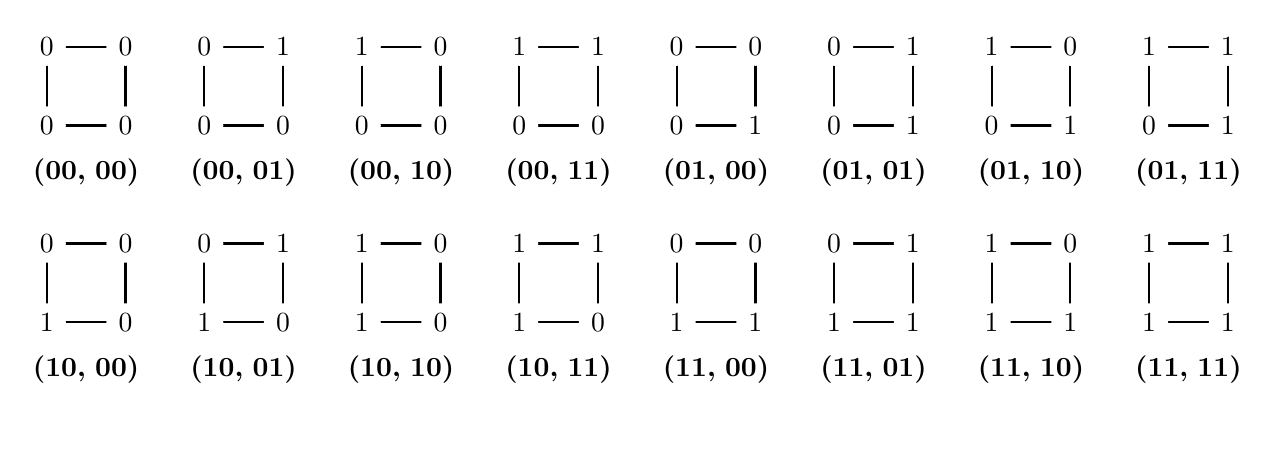
\begin{tikzpicture}
        % row1
        \cell{0}{-0.5}{1}{0.5}
        \cell{2}{-0.5}{3}{0.5}
        \cell{4}{-0.5}{5}{0.5}
        \cell{6}{-0.5}{7}{0.5}
        \cell{8}{-0.5}{9}{0.5}
        \cell{10}{-0.5}{11}{0.5}
        \cell{12}{-0.5}{13}{0.5}
        \cell{14}{-0.5}{15}{0.5}
        % row2
        \cell{0}{2}{1}{3}
        \cell{2}{2}{3}{3}
        \cell{4}{2}{5}{3}
        \cell{6}{2}{7}{3}
        \cell{8}{2}{9}{3}
        \cell{10}{2}{11}{3}
        \cell{12}{2}{13}{3}
        \cell{14}{2}{15}{3}

        % label for row 1
        \( \lablvertex{0}{-0.5}{$1$} \)
        \( \lablvertex{1}{-0.5}{$0$} \)
        \( \lablvertex{2}{-0.5}{$1$} \)
        \( \lablvertex{3}{-0.5}{$0$} \)
        \( \lablvertex{4}{-0.5}{$1$} \)
        \( \lablvertex{5}{-0.5}{$0$} \)
        \( \lablvertex{6}{-0.5}{$1$} \)
        \( \lablvertex{7}{-0.5}{$0$} \)
        \( \lablvertex{8}{-0.5}{$1$} \)
        \( \lablvertex{9}{-0.5}{$1$} \)
        \( \lablvertex{10}{-0.5}{$1$} \)
        \( \lablvertex{11}{-0.5}{$1$} \)
        \( \lablvertex{12}{-0.5}{$1$} \)
        \( \lablvertex{13}{-0.5}{$1$} \)
        \( \lablvertex{14}{-0.5}{$1$} \)
        \( \lablvertex{15}{-0.5}{$1$} \)
        
        % label for row 2
        \( \lablvertex{0}{0.5}{$0$} \)
        \( \lablvertex{1}{0.5}{$0$} \)
        \( \lablvertex{2}{0.5}{$0$} \)
        \( \lablvertex{3}{0.5}{$1$} \)
        \( \lablvertex{4}{0.5}{$1$} \)
        \( \lablvertex{5}{0.5}{$0$} \)
        \( \lablvertex{6}{0.5}{$1$} \)
        \( \lablvertex{7}{0.5}{$1$} \)
        \( \lablvertex{8}{0.5}{$0$} \)
        \( \lablvertex{9}{0.5}{$0$} \)
        \( \lablvertex{10}{0.5}{$0$} \)
        \( \lablvertex{11}{0.5}{$1$} \)
        \( \lablvertex{12}{0.5}{$1$} \)
        \( \lablvertex{13}{0.5}{$0$} \)
        \( \lablvertex{14}{0.5}{$1$} \)
        \( \lablvertex{15}{0.5}{$1$} \)

        % label for row 3
        \( \lablvertex{0}{2}{$0$} \)
        \( \lablvertex{1}{2}{$0$} \)
        \( \lablvertex{2}{2}{$0$} \)
        \( \lablvertex{3}{2}{$0$} \)
        \( \lablvertex{4}{2}{$0$} \)
        \( \lablvertex{5}{2}{$0$} \)
        \( \lablvertex{6}{2}{$0$} \)
        \( \lablvertex{7}{2}{$0$} \)
        \( \lablvertex{8}{2}{$0$} \)
        \( \lablvertex{9}{2}{$1$} \)
        \( \lablvertex{10}{2}{$0$} \)
        \( \lablvertex{11}{2}{$1$} \)
        \( \lablvertex{12}{2}{$0$} \)
        \( \lablvertex{13}{2}{$1$} \)
        \( \lablvertex{14}{2}{$0$} \)
        \( \lablvertex{15}{2}{$1$} \)
        
        % label for row 4
        \( \lablvertex{0}{3}{$0$} \)
        \( \lablvertex{1}{3}{$0$} \)
        \( \lablvertex{2}{3}{$0$} \)
        \( \lablvertex{3}{3}{$1$} \)
        \( \lablvertex{4}{3}{$1$} \)
        \( \lablvertex{5}{3}{$0$} \)
        \( \lablvertex{6}{3}{$1$} \)
        \( \lablvertex{7}{3}{$1$} \)
        \( \lablvertex{8}{3}{$0$} \)
        \( \lablvertex{9}{3}{$0$} \)
        \( \lablvertex{10}{3}{$0$} \)
        \( \lablvertex{11}{3}{$1$} \)
        \( \lablvertex{12}{3}{$1$} \)
        \( \lablvertex{13}{3}{$0$} \)
        \( \lablvertex{14}{3}{$1$} \)
        \( \lablvertex{15}{3}{$1$} \)

        % numbers row 1
        \( \lablnode{0.5}{1.4}{\textbf{(}$\mathbf{00}$\textbf{,} $\mathbf{00}$\textbf{)}} \)
        \( \lablnode{2.5}{1.4}{\textbf{(}$\mathbf{00}$\textbf{,} $\mathbf{01}$\textbf{)}} \)
        \( \lablnode{4.5}{1.4}{\textbf{(}$\mathbf{00}$\textbf{,} $\mathbf{10}$\textbf{)}} \)
        \( \lablnode{6.5}{1.4}{\textbf{(}$\mathbf{00}$\textbf{,} $\mathbf{11}$\textbf{)}} \)
        \( \lablnode{8.5}{1.4}{\textbf{(}$\mathbf{01}$\textbf{,} $\mathbf{00}$\textbf{)}} \)
        \( \lablnode{10.5}{1.4}{\textbf{(}$\mathbf{01}$\textbf{,} $\mathbf{01}$\textbf{)}} \)
        \( \lablnode{12.5}{1.4}{\textbf{(}$\mathbf{01}$\textbf{,} $\mathbf{10}$\textbf{)}} \)
        \( \lablnode{14.5}{1.4}{\textbf{(}$\mathbf{01}$\textbf{,} $\mathbf{11}$\textbf{)}} \)
        
        % numbers row 2
        \( \lablnode{0.5}{-1.1}{\textbf{(}$\mathbf{10}$\textbf{,} $\mathbf{00}$\textbf{)}} \)
        \( \lablnode{2.5}{-1.1}{\textbf{(}$\mathbf{10}$\textbf{,} $\mathbf{01}$\textbf{)}} \)
        \( \lablnode{4.5}{-1.1}{\textbf{(}$\mathbf{10}$\textbf{,} $\mathbf{10}$\textbf{)}} \)
        \( \lablnode{6.5}{-1.1}{\textbf{(}$\mathbf{10}$\textbf{,} $\mathbf{11}$\textbf{)}} \)
        \( \lablnode{8.5}{-1.1}{\textbf{(}$\mathbf{11}$\textbf{,} $\mathbf{00}$\textbf{)}} \)
        \( \lablnode{10.5}{-1.1}{\textbf{(}$\mathbf{11}$\textbf{,} $\mathbf{01}$\textbf{)}} \)
        \( \lablnode{12.5}{-1.1}{\textbf{(}$\mathbf{11}$\textbf{,} $\mathbf{10}$\textbf{)}} \)
        \( \lablnode{14.5}{-1.1}{\textbf{(}$\mathbf{11}$\textbf{,} $\mathbf{11}$\textbf{)}} \)
    \end{tikzpicture}
\end{center}

Next let $u_{(i,j)}$ be the number of tiles in $\mathbb{T}$ that can map to cell $(i,j)$. These values are simple to calculate, as each tile in $\mathbb{T}$ can only be part of a knot in certain ways. For example, $u_{(00, 01)} = 1$, as cell $(00,01)$ can only be formed by a mosaic with $T_3$ in that location. We can see that $u_{(01,10)}=4$, as cell $(01,10)$ can be from the $T_7,T_8,T_9$, or $T_{10}$ tiles. Finally, we have $u_{(00,00)}=11$, as any tile can fail to contribute to forming a knot. Table \ref{tbl:Preimage of binary cell lattice} summarizes the tiles in the preimage for each cell $(i,j)$. 

\begin{table}[h!]
    \begin{center}
        \begin{tabular}{ |c|l|c|c|l|c| } 
            \hline
            \textbf{Cell (}$\mathbf{i}$\textbf{,} $\mathbf{j}$\textbf{)} & \textbf{Preimage} & $\mathbf{u_{(i,j)}}$ & \textbf{Cell (}$\mathbf{i}$\textbf{,} $\mathbf{j}$\textbf{)} & \textbf{Preimage} & $\mathbf{u_{(i,j)}}$ \\ 
            \hline
            $(00, 00)$ & $\mathbb{T}$ & $11$ & $(10, 00)$ & $T_1$ & $1$ \\
            \hline
            $(00, 01)$ & $T_3$ & $1$ & $(10, 01)$ & $T_{7},T_{8},T_{9},T_{10}$ & $4$ \\
            \hline
            $(00, 10)$ & $T_4$ & $1$ & $(10, 10)$ & $T_6$ & $1$ \\
            \hline
            $(00, 11)$ & $T_5$ & $1$ & $(10, 11)$ & $T_2$ & $1$ \\
            \hline
            $(01, 00)$ & $T_2$ & $1$ & $(11, 00)$ & $T_5$ & $1$ \\
            \hline
            $(01, 01)$ & $T_6$ & $1$ & $(11, 01)$ & $T_4$ & $1$ \\
            \hline
            $(01, 10)$ & $T_{7},T_{8},T_{9},T_{10}$ & $4$ & $(11, 10)$ & $T_1$ & $1$ \\
            \hline
            $(01, 11)$ & $T_1$ & $1$ & $(11, 11)$ & $\mathbb{T}$ & $11$ \\
            \hline
        \end{tabular}
        \caption{Preimages of each unique cell}
        \label{tbl:Preimage of binary cell lattice}
    \end{center}
\end{table}

However, for some binary lattice $\ell$ the quantity 

\begin{equation}
    U(\ell) := \prod_{\text{Cell }(i,j) \in \ell} u_{(i,j)}
\end{equation}

is not necessarily equal to $\left|f^{-1}\left(\{\ell\}\right)\right|$, as $U(\ell)$ does not \textit{just} count the number of mosaics that map to $\ell$ under $f$. 

\begin{exmp}

Consider the following binary lattices for $s_{4,2}$. 

\begin{center}
    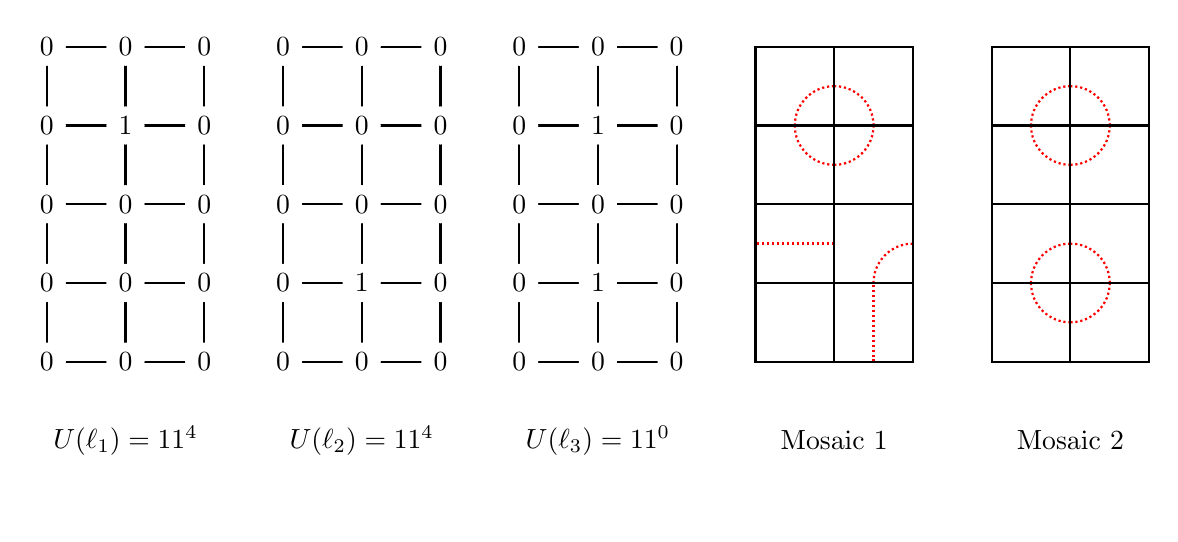
\begin{tikzpicture}

        % row1
        \cell{-3}{0}{-2}{1}
        \cell{-3}{1}{-2}{2}
        \cell{-3}{2}{-2}{3}
        \cell{-3}{3}{-2}{4}
        \cell{-2}{0}{-1}{1}
        \cell{-2}{1}{-1}{2}
        \cell{-2}{2}{-1}{3}
        \cell{-2}{3}{-1}{4}

        \( \lablnode{-2}{-1}{$U(\ell_{1}) = 11^4$} \)

        \( \lablvertex{-3}{0}{$0$} \)
        \( \lablvertex{-2}{0}{$0$} \)
        \( \lablvertex{-1}{0}{$0$} \)

        \( \lablvertex{-3}{1}{$0$} \)
        \( \lablvertex{-2}{1}{$0$} \)
        \( \lablvertex{-1}{1}{$0$} \)

        \( \lablvertex{-3}{2}{$0$} \)
        \( \lablvertex{-2}{2}{$0$} \)
        \( \lablvertex{-1}{2}{$0$} \)

        \( \lablvertex{-3}{3}{$0$} \)
        \( \lablvertex{-2}{3}{$1$} \)
        \( \lablvertex{-1}{3}{$0$} \)

        \( \lablvertex{-3}{4}{$0$} \)
        \( \lablvertex{-2}{4}{$0$} \)
        \( \lablvertex{-1}{4}{$0$} \)

        % row1
        \cell{0}{0}{1}{1}
        \cell{0}{1}{1}{2}
        \cell{0}{2}{1}{3}
        \cell{0}{3}{1}{4}
        \cell{1}{0}{2}{1}
        \cell{1}{1}{2}{2}
        \cell{1}{2}{2}{3}
        \cell{1}{3}{2}{4}

        \( \lablnode{1}{-1}{$U(\ell_{2}) =11^4$} \)
        
        \( \lablvertex{0}{0}{$0$} \)
        \( \lablvertex{1}{0}{$0$} \)
        \( \lablvertex{2}{0}{$0$} \)

        \( \lablvertex{0}{1}{$0$} \)
        \( \lablvertex{1}{1}{$1$} \)
        \( \lablvertex{2}{1}{$0$} \)

        \( \lablvertex{0}{2}{$0$} \)
        \( \lablvertex{1}{2}{$0$} \)
        \( \lablvertex{2}{2}{$0$} \)

        \( \lablvertex{0}{3}{$0$} \)
        \( \lablvertex{1}{3}{$0$} \)
        \( \lablvertex{2}{3}{$0$} \)

        \( \lablvertex{0}{4}{$0$} \)
        \( \lablvertex{1}{4}{$0$} \)
        \( \lablvertex{2}{4}{$0$} \)

        % row1
        \cell{3}{0}{4}{1}
        \cell{3}{1}{4}{2}
        \cell{3}{2}{4}{3}
        \cell{3}{3}{4}{4}
        \cell{4}{0}{5}{1}
        \cell{4}{1}{5}{2}
        \cell{4}{2}{5}{3}
        \cell{4}{3}{5}{4}

        \( \lablnode{4}{-1}{$U(\ell_{3}) = 11^0$} \)

        \( \lablvertex{3}{0}{$0$} \)
        \( \lablvertex{4}{0}{$0$} \)
        \( \lablvertex{5}{0}{$0$} \)

        \( \lablvertex{3}{1}{$0$} \)
        \( \lablvertex{4}{1}{$1$} \)
        \( \lablvertex{5}{1}{$0$} \)

        \( \lablvertex{3}{2}{$0$} \)
        \( \lablvertex{4}{2}{$0$} \)
        \( \lablvertex{5}{2}{$0$} \)

        \( \lablvertex{3}{3}{$0$} \)
        \( \lablvertex{4}{3}{$1$} \)
        \( \lablvertex{5}{3}{$0$} \)

        \( \lablvertex{3}{4}{$0$} \)
        \( \lablvertex{4}{4}{$0$} \)
        \( \lablvertex{5}{4}{$0$} \)

        \cell{6}{0}{7}{1}
        \cellF{7}{0}{8}{1}

        \cellE{6}{1}{7}{2}
        \cellB{7}{1}{8}{2}

        \cellC{6}{2}{7}{3}
        \cellD{7}{2}{8}{3}    

        \cellB{6}{3}{7}{4}
        \cellA{7}{3}{8}{4}    

        \( \lablnode{7}{-1}{Mosaic $1$} \)

        \cellC{9}{0}{10}{1}
        \cellD{10}{0}{11}{1}

        \cellB{9}{1}{10}{2}
        \cellA{10}{1}{11}{2}

        \cellC{9}{2}{10}{3}
        \cellD{10}{2}{11}{3}    

        \cellB{9}{3}{10}{4}
        \cellA{10}{3}{11}{4}    

        \( \lablnode{10}{-1}{Mosaic $2$} \)

    \end{tikzpicture}
\end{center}

$U(\ell_{1})$ uniquely counts Mosaic $1$, but both $U(\ell_{1})$ and $U(\ell_{2})$ count Mosaic $2$, for which $f(\text{Mosaic } 2) = \ell_3$. This is because each cell in the bottom two rows of $(00,00)$ cells in $\ell_1$ could have come from $11$ possible cells, though $1$ of those $11^4$ permutations contains a new knot. 

\label{exmp:U doesnt work}
\end{exmp}

\begin{definition}
    A knot is \textit{specified} by a binary lattice $\ell$ if all mosaics in $f^{-1}(\{\ell\})$ contain the knot.
\end{definition}

\begin{exmp}
    From Example \ref{exmp:U doesnt work}, $\ell_1$ specifies the knot in the top $2$ rows of Mosaic $1$ and Mosaic $2$, but not the knot in the bottom $2$ rows of Mosaic $2$. $\ell_3$ specifies both knots in Mosaic $2$.
\label{exmp:specifying example}
\end{exmp}

\begin{definition}
    Let $K: \mathbb{L}^{(m,n)} \to \mathbb{N}$ be the number of knots specified in $\ell$.
\end{definition}

\begin{exmp}
    From Example \ref{exmp:U doesnt work}, $K(\ell_1) =1$, $K(\ell_2) =1$,  and $K(\ell_3) =2$.

\label{exmp:counting knots}
\end{exmp}

\begin{definition}
For a binary lattice $\ell$, let $\mathbb{U}(\ell)$ be the set of binary lattices whose preimage mosaics under $f$ are counted by $U(\ell)$. A binary lattice $\ell'$ is in $\mathbb{U}(\ell)$ if one can replace either some number of $(00,00)$ or $(11,11)$ cells in $\ell$ with other cells in $C$ to create $\ell'$. This corresponds with specifying new knots in the mosaics in the preimage of $\ell$ while leaving all knots specified by $\ell$ unchanged. 
\end{definition}

\begin{exmp}
From Example \ref{exmp:U doesnt work}, $\mathbb{U}(\ell_1) = \{\ell_1, \ell_3\}$, $\mathbb{U}(\ell_2) = \{\ell_2, \ell_3\}$, and $\mathbb{U}(\ell_3) = \{\ell_3\}$.

% $$\left|f^{-1}(\{\ell_1,\ell_2,\ell_3\})\right| = \left|f^{-1}(\mathbb{U}(\ell_1) \cup \mathbb{U}(\ell_2) \cup \mathbb{U}(\ell_3))\right| = U(\ell_1) + U(\ell_2) - U(\ell_3).$$

\label{exmp:four two mosaics}
\end{exmp}

From the definition of $\mathbb{U}$, we have

\begin{equation}
    U(\ell) = \sum_{\ell' \in \mathbb{U}(\ell)}|f^{-1}(\ell')|.
    \label{eq:U identity}
\end{equation}

Therefore $s_{m,n} \neq \sum_{\ell \in \mathbb{L}^{(m,n)}} U(\ell)$, as the sum overcounts mosaics for all $\ell$ that have $\mathbb{U}(\ell) \neq \{\ell\}$. 

\begin{definition}
    Let $\ell^* \in \mathbb{L}^{(m,n)}$ be the binary lattice made up of all $(00,00)$ cells.
    \label{def:all zeros}
\end{definition}

$\ell^*$ specifies $0$ knots and has $U(\ell^*) = 11^{mn} = \left|\mathbb{M}^{(m,n)}\right|$, which clearly overcounts $s_{m,n}$. Also note that $\mathbb{U}(\ell^*) = \mathbb{L}^{(m,n)}$.


\begin{prop}
    By regrouping terms we have

    \begin{equation}
        \sum_{\ell \in \mathbb{L}^{(m,n)}} U(\ell) = \sum_{\ell \in \mathbb{L}^{(m,n)}}\sum_{\ell' \in \mathbb{U}(\ell)}|f^{-1}(\ell')| = \sum_{\ell \in \mathbb{L}^{(m,n)}} \left(\binom{K(\ell)}{0} + \dots + \binom{K(\ell)}{K(\ell)}\right)|f^{-1}(\ell)|.
        \label{eq:double counting terms}
    \end{equation}
\end{prop}

\begin{proof}
    The first equality follows directly from Equation \ref{eq:U identity}. For the second equality, notice that the number of times $|f^{-1}(\ell)|$ appears in the second sum of Equation \ref{eq:double counting terms} is the number of times a binary lattice $\ell$ appears in the set

    $$\bigcup_{\ell \in \mathbb{L}^{(m,n)}} \{\mathbb{U}(\ell)\}.$$
    
    If $\ell$ has $K(\ell)>0$, the definition of $\mathbb{U}$ gives that $\ell$ appears once in the $\mathbb{U}$ set for the binary lattice that specifies $0$ knots (ie. $\ell^*$). $\ell$ also appears in the $\mathbb{U}$ set for each binary lattice that specifies $1$ of the knots in $\ell$. $\ell$ also appears in the $\mathbb{U}$ set for each binary lattice that specifies $2$ of the knots in $\ell$, and so on up to specifying $K(\ell)$ knots. As the number of ways $k \leq K(\ell)$ knots can specify $K(\ell)$ knots are the binomial coefficients, this gives the second equality for all $\ell \neq \ell^*$.

    If $\ell = \ell^*$, we have that $K(\ell^*)=0$, so $|f^{-1}(\ell^*)|$ is only counted once. As $\binom{0}{0}=1$, this completes the proof.
\end{proof}

\begin{prop}
    The number of mosaics of size $(m,n)$ that do not contain a knot $s_{m,n}$ has

    \begin{equation}
    s_{m,n} = \sum_{\ell \in \mathbb{L}^{(m,n)}} (-1)^{K(\ell)} U(\ell).
    \label{eq:ugly inc excl}
    \end{equation}
\end{prop}

\begin{proof}
    By the binomial theorem,
    
    $$0 = (1-1)^{K(\ell)} = \left(\binom{K(\ell)}{0} - \binom{K(\ell)}{1} + \dots + (-1)^{K(\ell)}\binom{K(\ell)}{K(\ell)}\right),$$
    
    so if we group terms as in Equation \ref{eq:double counting terms}, we get that all terms where $\ell \neq \ell^*$ are $0$. Therefore, 
    
    $$\sum_{\ell \in \mathbb{L}^{(m,n)}} (-1)^{K(\ell)} U(\ell) = \binom{0}{0}|f^{-1}(\ell^*)| = s_{m,n}.$$
\end{proof}

It is important to note here that a knot that contains tiles $T_7$ or $T_8$ can appear to be two separate knots which we consider as $1$ knot.

\begin{exmp}
Figure \ref{fig:messy multi knot} shows a mosaic that appears to have $2$ knots, but we only consider as $1$ knot. A rule of thumb that can be followed is if knots that contain $T_7$ or $T_8$ tiles can be replaced by $T_9$ or $T_{10}$ tiles to form a single knot, then the original ``knots" we consider as $1$ knot.

\begin{figure}[h!]
\begin{center}

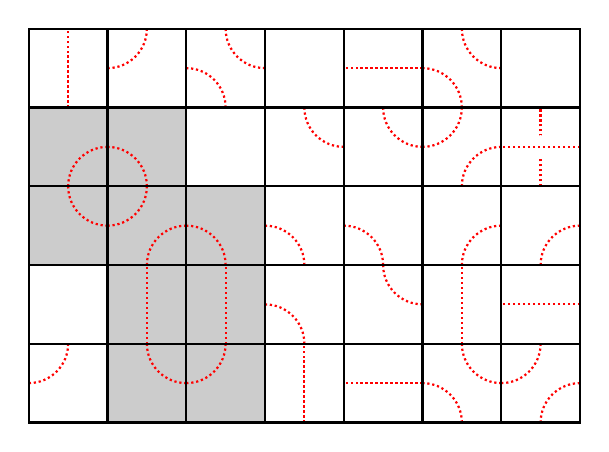
\begin{tikzpicture}
    % row1
    \cellD{0}{0}{1}{1}
    \cellCf{1}{0}{2}{1}
    \cellDf{2}{0}{3}{1}
    \cellF{3}{0}{4}{1}
    \cellE{4}{0}{5}{1}
    \cellG{5}{0}{6}{1}
    \cellH{6}{0}{7}{1}
    % row2
    \cell{0}{1}{1}{2}
    \cellFf{1}{1}{2}{2}
    \cellFf{2}{1}{3}{2}
    \cellA{3}{1}{4}{2}
    \cellC{4}{1}{5}{2}
    \cellF{5}{1}{6}{2}
    \cellE{6}{1}{7}{2}
    % row3
    \cellCf{0}{2}{1}{3}
    \cellHf{1}{2}{2}{3}
    \cellAf{2}{2}{3}{3}
    \cellA{3}{2}{4}{3}
    \cellA{4}{2}{5}{3}
    \cellB{5}{2}{6}{3}
    \cellB{6}{2}{7}{3}
    % row4
    \cellBf{0}{3}{1}{4}
    \cellAf{1}{3}{2}{4}
    \cell{2}{3}{3}{4}
    \cellC{3}{3}{4}{4}
    \cellC{4}{3}{5}{4}
    \cellH{5}{3}{6}{4}
    \cellI{6}{3}{7}{4}
    % row5
    \cellF{0}{4}{1}{5}
    \cellD{1}{4}{2}{5}
    \cellG{2}{4}{3}{5}
    \cell{3}{4}{4}{5}
    \cellE{4}{4}{5}{5}
    \cellG{5}{4}{6}{5}
    \cell{6}{4}{7}{5}
\end{tikzpicture}

\end{center}
\caption{A messy knot mosaic with $1$ knot}
\label{fig:messy multi knot}
\end{figure}

\end{exmp}

\section{A Cell-Level Identity}

Though Equation \ref{eq:ugly inc excl} does compute $s_{m,n}$, computing the number of knots specified in a binary lattice $K(\ell)$ requires examining the entire, global structure of $\ell$. It will be more efficient to recover the $(-1)^{K(\ell)}$ term at the cell level. The idea is to add a coefficient $p_{(i,j)}$ to each value of $u_{(i,j)}$ so that the $(-1)^{K(\ell)}$ term is recovered.

\begin{condition}
    A subset of cells $\mathcal{K}$ in a binary lattice $\ell$ meets this condition if
    
    \begin{equation}
        \prod_{\text{Cell } (i,j) \in \mathcal{K}} p_{(i,j)} = -1,
        \label{eq:neg prod knot condition}
    \end{equation}
    with $p_{(i,j)} \in \{-1,1\}$.
    \label{cond:neg prod condition}
\end{condition}

By the definition of $K(\ell)$, if there exists values $p_{(i,j)}$ for which Condition \ref{cond:neg prod condition} holds only for cells $\mathcal{K}$ that specify a knot, then the $(-1)^{K(\ell)}$ is recovered at the cell level.

\begin{prop}
    There exists values $p_{(i,j)}$ for which Condition \ref{cond:neg prod condition} holds for any set of cells that specify a knot.
    \label{prop:neg prod prop}
\end{prop}

\begin{proof}

We can immediately see $p_{(00,00)} = p_{(11,11)} = 1$, as cells $(00,00)$ and $(11,11)$ can never be in the collection of cells that specify a knot, and so must be positive.

For the remaining values of $p_{(i,j)}$, we examine the cells that map to the smallest knot, shown in Figure \ref{fig:smallest knot}. 

\begin{figure}[h!]
\begin{center}
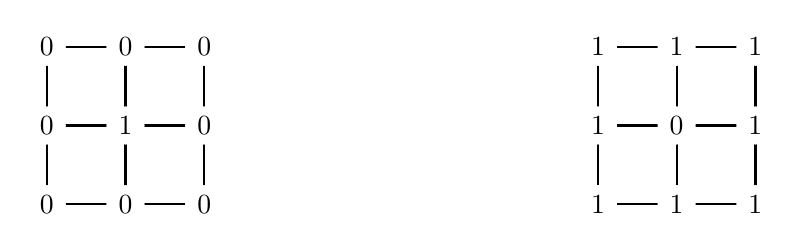
\begin{tikzpicture}
    % row1
    \cell{0}{0}{1}{1}
    \cell{1}{0}{2}{1}
    % row2
    \cell{0}{1}{1}{2}
    \cell{1}{1}{2}{2}
    % label for row1
    \( \lablvertex{0}{0}{$0$} \)
    \( \lablvertex{1}{0}{$0$} \)
    \( \lablvertex{2}{0}{$0$} \)
    % label for row2
    \( \lablvertex{0}{1}{$0$} \)
    \( \lablvertex{1}{1}{$1$} \)
    \( \lablvertex{2}{1}{$0$} \)
    % label for row3
    \( \lablvertex{0}{2}{$0$} \)
    \( \lablvertex{1}{2}{$0$} \)
    \( \lablvertex{2}{2}{$0$} \)

    % \( \lablnode{1}{-0.5}{$p_{(00,01)} p_{(00,10)} p_{(01,00)} p_{(10,00)} = -1$} \)

    % row1
    \cell{7}{0}{8}{1}
    \cell{8}{0}{9}{1}
    % row2
    \cell{7}{1}{8}{2}
    \cell{8}{1}{9}{2}
    % label for row1
    \( \lablvertex{7}{0}{$1$} \)
    \( \lablvertex{8}{0}{$1$} \)
    \( \lablvertex{9}{0}{$1$} \)
    % label for row2
    \( \lablvertex{7}{1}{$1$} \)
    \( \lablvertex{8}{1}{$0$} \)
    \( \lablvertex{9}{1}{$1$} \)
    % label for row3
    \( \lablvertex{7}{2}{$1$} \)
    \( \lablvertex{8}{2}{$1$} \)
    \( \lablvertex{9}{2}{$1$} \)
    
    % \( \lablnode{8}{-0.5}{$p_{(11,10)} p_{(11,01)} p_{(10,11)} p_{(01,11)} = -1$} \)
\end{tikzpicture}
\end{center}
\caption{Portions of binary lattices associated with the smallest knot}
\label{fig:constraints i and ii}
\end{figure}

Condition \ref{cond:neg prod condition} amounts to the following two equations

\begin{equation}
  \begin{aligned}
  p_{(00,01)} p_{(00,10)} p_{(01,00)} p_{(10,00)} & = -1  \\
  p_{(11,10)} p_{(11,01)} p_{(10,11)} p_{(01,11)} & = -1,
  \end{aligned}
  \label{eq:constraints i and ii}
\end{equation}

one for each portion of a binary lattice in Figure \ref{fig:constraints i and ii}. We refer to the equations above as \textit{constraints}, as they constrain the possible assignments of $p_{(i,j)}$. Let the constraints in Equation \ref{eq:constraints i and ii} be numbered $1$ and $2$.

To define the remaining constraints, we next examine how specified knots arise in binary lattices.

\begin{definition}
    A subset of vertices $X$ in a binary lattice $\ell$ is said to be \textit{connected} if all vertices are the same value, and for any pair of vertices $x_1, x_2 \in X$ there exists a path between $x_1$ and $x_2$ of unit vertical, horizontal, and diagonal moves so that all of vertices in the path are in $X$. 
\end{definition}

In a binary lattice, a specified knot corresponds with a set of connected $0$ or $1$ vertices, that if $0$ are not connected to the boundary $0$'s. This is illustrated in Figure \ref{fig:example of f mapping}, where the $3$ knots correspond with $3$ edge-and-corner connected regions, excluding the region that is connected to the boundary. 

The idea is, starting with a single vertex labeled $1$, we can construct an arbitrary set of connected vertices labeled $1$ by continually flipping a neighboring $0$s to $1$s. This \textit{bit flip} operation, depicted in Figure \ref{fig:bit flip}, corresponds with changing the identity of the four cells that share that vertex.

As each cell has its associated $p_{(i,j)}$ value, it must be the case that the bit flip preserves Condition \ref{cond:neg prod condition} for the cells involved. Additionally, as the surrounding $8$ vertices are unchanged, this creates $2^8$ constraints. In each of these constraints, the parity of the number of connected regions of $1$s must either change or stay the same after the bit flip. If the parity remains unchanged, the bit flip is of \textit{Type 1}, and if the parity changes the bit flip is of \textit{Type 2}.

\begin{figure}[h!]
    \begin{center}

\begin{subfigure}{0.4\textwidth}
    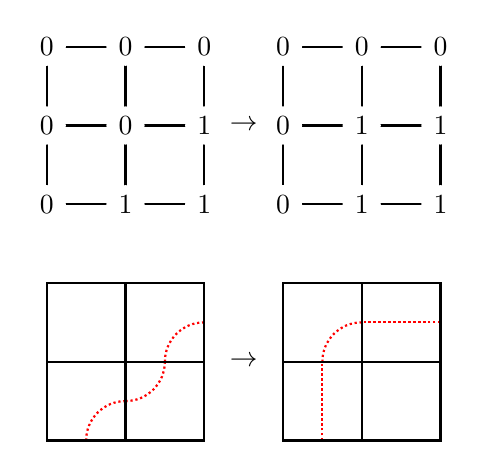
\begin{tikzpicture}
        % row1
        \cell{0}{0}{1}{1}
        \cell{1}{0}{2}{1}
        % row2
        \cell{0}{1}{1}{2}
        \cell{1}{1}{2}{2}
        % label for row1
        \( \lablvertex{0}{0}{$0$} \)
        \( \lablvertex{1}{0}{$1$} \)
        \( \lablvertex{2}{0}{$1$} \)
        % label for row2
        \( \lablvertex{0}{1}{$0$} \)
        \( \lablvertex{1}{1}{$0$} \)
        \( \lablvertex{2}{1}{$1$} \)
        % label for row3
        \( \lablvertex{0}{2}{$0$} \)
        \( \lablvertex{1}{2}{$0$} \)
        \( \lablvertex{2}{2}{$0$} \)
        % row1
        \cell{3}{0}{4}{1}
        \cell{4}{0}{5}{1}
        % row2
        \cell{3}{1}{4}{2}
        \cell{4}{1}{5}{2}
        % label for row1
        \( \lablvertex{3}{0}{$0$} \)
        \( \lablvertex{4}{0}{$1$} \)
        \( \lablvertex{5}{0}{$1$} \)
        % label for row2
        \( \lablvertex{3}{1}{$0$} \)
        \( \lablvertex{4}{1}{$1$} \)
        \( \lablvertex{5}{1}{$1$} \)
        % label for row3
        \( \lablvertex{3}{2}{$0$} \)
        \( \lablvertex{4}{2}{$0$} \)
        \( \lablvertex{5}{2}{$0$} \)

        \( \lablnode{2.5}{1}{$\rightarrow$} \)
        
        \cellB{0}{-3}{1}{-2}
        \cellD{1}{-3}{2}{-2}
        \cell{0}{-2}{1}{-1}
        \cellB{1}{-2}{2}{-1}
        
        \( \lablnode{2.5}{-2}{$\rightarrow$} \)

        \cellF{3}{-3}{4}{-2}
        \cell{4}{-3}{5}{-2}
        \cellB{3}{-2}{4}{-1}
        \cellE{4}{-2}{5}{-1}

    \end{tikzpicture}
    \caption{Type 1 bit flip and associated tiles}
    \label{fig:type 1 bit flip}
\end{subfigure}
% \hfill
\hspace{0.05\textwidth}
\begin{subfigure}{0.4\textwidth}
    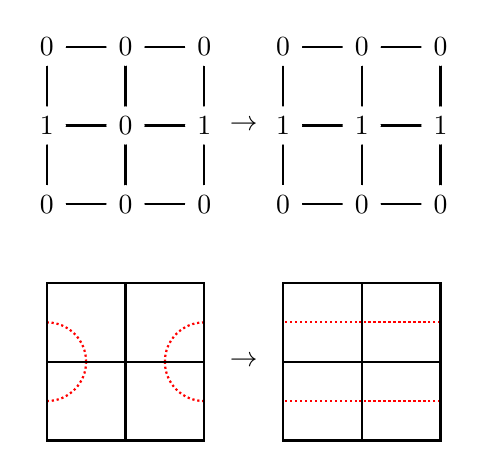
\begin{tikzpicture}
        % row1
        \cell{0}{0}{1}{1}
        \cell{1}{0}{2}{1}
        % row2
        \cell{0}{1}{1}{2}
        \cell{1}{1}{2}{2}
        % label for row1
        \( \lablvertex{0}{0}{$0$} \)
        \( \lablvertex{1}{0}{$0$} \)
        \( \lablvertex{2}{0}{$0$} \)
        % label for row2
        \( \lablvertex{0}{1}{$1$} \)
        \( \lablvertex{1}{1}{$0$} \)
        \( \lablvertex{2}{1}{$1$} \)
        % label for row3
        \( \lablvertex{0}{2}{$0$} \)
        \( \lablvertex{1}{2}{$0$} \)
        \( \lablvertex{2}{2}{$0$} \)
        
        % row1
        \cell{3}{0}{4}{1}
        \cell{4}{0}{5}{1}
        % row2
        \cell{3}{1}{4}{2}
        \cell{4}{1}{5}{2}
        % label for row1
        \( \lablvertex{3}{0}{$0$} \)
        \( \lablvertex{4}{0}{$0$} \)
        \( \lablvertex{5}{0}{$0$} \)
        % label for row2
        \( \lablvertex{3}{1}{$1$} \)
        \( \lablvertex{4}{1}{$1$} \)
        \( \lablvertex{5}{1}{$1$} \)
        % label for row3
        \( \lablvertex{3}{2}{$0$} \)
        \( \lablvertex{4}{2}{$0$} \)
        \( \lablvertex{5}{2}{$0$} \)

        \( \lablnode{2.5}{1}{$\rightarrow$} \)

        \cellD{0}{-3}{1}{-2}
        \cellC{1}{-3}{2}{-2}
        \cellA{0}{-2}{1}{-1}
        \cellB{1}{-2}{2}{-1}
        
        \( \lablnode{2.5}{-2}{$\rightarrow$} \)

        \cellE{3}{-3}{4}{-2}
        \cellE{4}{-3}{5}{-2}
        \cellE{3}{-2}{4}{-1}
        \cellE{4}{-2}{5}{-1}

    \end{tikzpicture}
    \caption{Type 2 bit flip and associated tiles}
    \label{fig:type 2 bit flip}
\end{subfigure}

\end{center}
\caption{Bit flips for binary lattices}
\label{fig:bit flip}
\end{figure}

For a bit flip of \textit{Type 1}, to adhere to Condition \ref{cond:neg prod condition}, the associated constraint is that the sign of the product of the related cells must stay the same after the flip. For example, Figure \ref{fig:type 1 bit flip} represents the constraint

\begin{equation}
    p_{(00,00)}p_{(00,01)}p_{(00,01)}p_{(01,11)} = p_{(00,01)}p_{(00,11)}p_{(01,01)}p_{(01,11)}.
\end{equation}

For a bit flip of \textit{Type 2}, to adhere to Condition \ref{cond:neg prod condition}, the associated constraint is that the sign of the product of the related cells must change after the flip. For example, Figure \ref{fig:type 2 bit flip} represents the constraint\footnote{In Figure \ref{fig:type 2 bit flip} the transformation corresponds with \textit{either} two distinct knot joining into one knot \textit{or} one knot splitting into two distinct knot. In either case, we want the sign of the product to change.}

\begin{equation}
    p_{(00,10)}p_{(00,01)}p_{(10,00)}p_{(01,00)} = -p_{(00,11)}p_{(00,11)}p_{(11,00)}p_{(11,00)}.
\end{equation}

This defines a procedure to define the $2^8$ bit flip constraints on $p_{(i,j)}$. We can then use software to verify that all $2^8 +2$ constraints admit a solution.

% We can then calculate the  Gröbner basis of the system to arrive at

% All unsimplified Type 1 and Type 2 constraints can be found in the Appendix.

\end{proof}

If we let $v_{(i,j)} := p_{(i,j)}u_{(i,j)},$ and similarly define

$$V(\ell) := \prod_{\text{Cell } (i,j) \in \ell} v_{(i,j)},$$

Proposition \ref{prop:neg prod prop} allows us to rewrite the term in the sum of Equation \ref{eq:ugly inc excl} to

\begin{equation}
    (-1)^{K(\ell)}U(\ell) = V(\ell) = \prod_{\text{Cell }(i,j) \in \ell} p_{(i,j)}u_{(i,j)} \text{ $\forall \ell$}.
    \label{eq:term fix}
\end{equation}

We summarize the values of $v_{(i,j)}$ in Table \ref{tbl:values of p and v}.

\begin{table}[h!]
    \begin{center}
        \begin{tabular}{ |c|r|r|r|c|r|r|r| } 
            \hline
            \textbf{Cell (}$\mathbf{i}$\textbf{,} $\mathbf{j}$\textbf{)} & $\mathbf{u_{(i,j)}}$ & $\mathbf{p_{(i,j)}}$ & $\mathbf{v_{(i,j)}}$ & \textbf{Cell (}$\mathbf{i}$\textbf{,} $\mathbf{j}$\textbf{)} & $\mathbf{u_{(i,j)}}$ & $\mathbf{p_{(i,j)}}$ & $\mathbf{v_{(i,j)}}$ \\ 
            \hline
            $(00, 00)$ & $11$ & $1$ & $11$ & $(10, 00)$ & $1$ & $-1$ & $-1$ \\
            \hline
            $(00, 01)$ & $1$ & $1$ & $1$ & $(10, 01)$ & $4$ & $1$ & $4$ \\
            \hline
            $(00, 10)$ & $1$ & $1$ & $1$ & $(10, 10)$ & $1$ & $1$ & $1$ \\
            \hline
            $(00, 11)$ & $1$ & $1$ & $1$ & $(10, 11)$ & $1$ & $1$ & $1$ \\
            \hline
            $(01, 00)$ & $1$ & $1$ & $1$ & $(11, 00)$ & $1$ & $1$ & $1$ \\
            \hline
            $(01, 01)$ & $1$ & $1$ & $1$ & $(11, 01)$ & $1$ & $1$ & $1$ \\
            \hline
            $(01, 10)$ & $4$ & $-1$ & $-4$ & $(11, 10)$ & $1$ & $-1$ & $-1$ \\
            \hline
            $(01, 11)$ & $1$ & $1$ & $1$ & $(11, 11)$ & $11$ & $1$ & $11$ \\
            \hline
        \end{tabular}
        \caption{Values of $p_{(i,j)}$ and $v_{(i,j)}$}
        \label{tbl:values of p and v}
    \end{center}
\end{table}

Equation \ref{eq:term fix} allows us to simplify Equation \ref{eq:ugly inc excl} to

\begin{equation}
    s_{m,n} = \sum_{\ell \in \mathbb{L}^{(m,n)}} \prod_{\text{Cell }(i,j) \in \ell} v_{(i,j)}.
\label{eq:technically correct}
\end{equation}

$s_{m,n}$ can be calculated more efficiently than in Equation \ref{eq:technically correct} using the state matrix recursion introduced in \cite{Oh2014}.

\section{Proof of Theorem \ref{thm: messy mosaics}}

This argument generally follows the proof in \cite{Oh2014}.

Let a \textit{binary sub-lattice} of size $(p,q)$ be a rectangular lattice of $p+1$ by $q+1$ vertices, in which only the left and right boundary vertices must be labeled $0$, and all other vertices can be labeled $0$ or $1$. Also let $\hat{\mathbb{L}}^{(p,q)}$ be the set of all binary sub-lattices of size $(p,q)$. We choose a similar indexing convention for binary sub-lattices as individual cells, in which we, ignoring the first and last $0$, read the bottom row and the top row as two binary numbers $(i,j)$ respectively. For example, Figure \ref{fig:binary sub lattice example} is a binary sub-lattice of size $(2,4)$ with index $(011,100)$.

\begin{figure}[h!]
    \begin{center}
    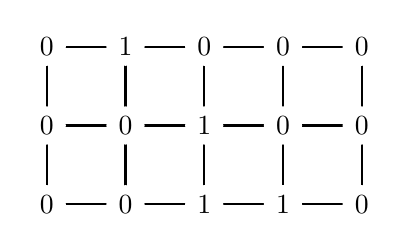
\begin{tikzpicture}
        % row 1
        \cell{0}{0}{1}{1}
        \cell{1}{0}{2}{1}
        \cell{2}{0}{3}{1}
        \cell{3}{0}{4}{1}
        % row 2
        \cell{0}{1}{1}{2}
        \cell{1}{1}{2}{2}
        \cell{2}{1}{3}{2}
        \cell{3}{1}{4}{2}

        \( \lablvertex{0}{0}{$0$} \)
        \( \lablvertex{1}{0}{$0$} \)
        \( \lablvertex{2}{0}{$1$} \)
        \( \lablvertex{3}{0}{$1$} \)
        \( \lablvertex{4}{0}{$0$} \)

        \( \lablvertex{0}{1}{$0$} \)
        \( \lablvertex{1}{1}{$0$} \)
        \( \lablvertex{2}{1}{$1$} \)
        \( \lablvertex{3}{1}{$0$} \)
        \( \lablvertex{4}{1}{$0$} \)

        \( \lablvertex{0}{2}{$0$} \)
        \( \lablvertex{1}{2}{$1$} \)
        \( \lablvertex{2}{2}{$0$} \)
        \( \lablvertex{3}{2}{$0$} \)
        \( \lablvertex{4}{2}{$0$} \)
    \end{tikzpicture}
    \end{center}
\caption{A binary sub-lattice of size $(2,4)$ with index $(011,100)$}
\label{fig:binary sub lattice example}
\end{figure}

As with binary lattices, we can compute $V(\hat{\ell})$ for a binary sub-lattice $\hat{\ell} \in \hat{\mathbb{L}}^{(p,q)}$.

We can now define the \textit{state matrix} for $\hat{\mathbb{L}}^{(p,q)}$ to be the $2^{q} \times 2^{q}$ matrix $A^{(p,q)} = (A_{i,j})$ where element 

$$A_{i,j} = \sum_{\hat{\ell}\text{ with index } (i,j)}V(\hat{\ell}).$$

Here we $A_{i,j}$ is the entry in the $i$-th row read top-to-bottom, and in the $j$-th column read left-to-right. As binary sub-lattices $\hat{\mathbb{L}}^{(p,q)}$ with index $(0\dots0,0\dots0)$ are just binary lattices, we have for a state matrix $A^{(p,q)}$ that 

$$A_{0,0} = \sum_{\ell \in \mathbb{L}^{(p,q)}}V(\ell).$$

Theorem \ref{thm: messy mosaics} amounts to an efficient procedure to compute $A^{(p,q)}$.

\begin{prop}
For the set $\hat{\mathbb{L}}^{(1,q)}$ the associated state matrix $A^{(1,q)}$ can be computed by first defining $A^{(1,2)} = \begin{bmatrix}
11^2 & 1 \\
-1 & 1
\end{bmatrix}$. We recursively define $A^{(1,q)} \in \mathbb{N}^{2^{q} \times 2^{q}}$ given $A^{(1,q-1)}$. Begin by writing
$
A^{(1,k)} = \begin{bmatrix}
A_{[0,0]} & A_{[0,1]} \\
A_{[1,0]} & A_{[1,1]}
\end{bmatrix}
$, where the block matrices $A_{[i,j]}$ are square block matrices of size $2^{k-1} \times 2^{k-1}$. We then have

$$
A^{(1,k+1)} = \begin{bmatrix*}[r]
    11A_{[0,0]} & 11^{-1}A_{[0,0]} & 11A_{[0,1]} & A_{[0,1]} \\
    -11^{-1}A_{[0,0]} & 11^{-1}A_{[0,0]} & 4A_{[0,1]} & A_{[0,1]} \\
    11A_{[1,0]} & -4A_{[1,0]} & 11A_{[1,1]}  & A_{[1,1]} \\
    A_{[1,0]} & -A_{[1,0]} & A_{[1,1]} & 11A_{[1,1]} \\
\end{bmatrix*}.
$$

Construct $A^{(1,q)}$ by starting with $k=2$ and recursing until $k=q$. 

\end{prop}

\begin{proof}
    \textbf{TODO}

    We use induction on $q$. We can immediately calculate $A^{(1,2)}$ by computing the values of $V$ for each $(1,2)$ sub-lattice. 
\end{proof}

\begin{prop}
    For the set $\mathbb{L}^{(p,q)}$, the state matrix has
    $$A^{(p,q)} = (A^{(1,q)})^p.$$
\end{prop}

\begin{proof}
    \textbf{TODO}
    
    We use induction on $p$. 
\end{proof}

\textbf{TODO}



\section{Extensions}
\label{section: Extensions}

Hong and Oh \cite{Hong2018} study the mosaic system with the tile set $\mathbb{T}^* = \{T_0, \dots,T_7\}$. This tile set constructs shapes we call \textit{polygons}\footnote{Polygons are more commonly called "self-avoiding polygons" in the literature to emphasize their relationship with self-avoiding walks.}. If we let $p_{m,n}$ be the number of polygon mosaics of size $(m,n)$, Hong and Oh showed the following results\footnote{The authors did not consider the mosaic containing all $T_0$ tiles a polygon mosaic, and so define $p_{m,n}$ as one less than what we define.}. 

\begin{thm}[\cite{Hong2018}]
    \label{thm:Hong2018}
    The number of polygon mosaics of size $(m,n)$ $p_{m,n}$ for $m,n \geq 2$ has

    $$2^{m+n-3} \left(\frac{17}{10}\right)^{(m-2)(n-2)} \leq p_{m,n} \leq 2^{m+n-3} \left(\frac{31}{16}\right)^{(m-2)(n-2)}.$$
\end{thm}

Though not stated in Hong and Oh \cite{Hong2018}, $p_{m,n}$ is exactly enumerated by Theorem \ref{thm:Oh2014} by replacing the $4$ in the definition of $O_{k+1}$ with a $0$.The array $p_{n,m}$ is A181245 on the OEIS \cite[OEIS]{oeis}. 

\textbf{TODO}

\section{Acknowledgements}

The authors would like to thank Michael Maltenfort for the edits, improvements and ideas for this paper. 

\newpage

\printbibliography

\section{Appendix}

\textbf{TODO}

\end{document}